\appendix
\addcontentsline{toc}{section}{Appendici}
\section*{Appendici}
\section{Resoconto delle attività di verifica}
Questa sezione riporta il resoconto delle attività di verifica svolte prima di ciascuna delle quattro revisioni stabilite dal committente (Revisione dei Requisiti, R. di Progettazione, R. di Qualifica e R. di Accettazione).
Al termine di ogni revisione il committente segnalerà le problematiche riscontrate attraverso una valutazione globale dell'andamento del progetto ed una dettagliata per ciascun documento, permettendo al gruppo di eliminare problemi e criticità nel progetto per poi procedere su una base verificata e il più possibile corretta.

\subsection{Revisione dei Requisiti}
In questa sezione vengono riportati gli esiti delle metriche relative ai processi e ai documenti durante la fase di Analisi.
\subsubsection{Qualità di processo}
\paragraph{Esiti metriche di processo} \MiniSpazio
\renewcommand{\arraystretch}{1.5}
\begin{table}[H]
	\begin{center}
		\begin{tabular}{|c|c|c|}
			\hline
			\rowcolor{title_row}
			\textbf{\color{title_text}{Metrica}} & \textbf{\color{title_text}{Valore ottenuto}} & \textbf{\color{title_text}{Esito}} \\
			\hline
			{Schedule Variance} & {0} & {Superato}\\	
			\hline
			{Budget Variance} & {-2.5\%} & {Superato}\\	
			\hline
		\end{tabular}
	\caption[Esiti metriche di processo, Analisi]{Esiti derivanti dall'applicazione delle metriche di processo}	
	\label{tabella: esiti derivanti dall'applicazione delle metriche di processo}
	\end{center}
\end{table}
\renewcommand{\arraystretch}{1}
\paragraph{Dettaglio delle verifiche tramite analisi} \Spazio
Il grafico rappresentante l'applicazione del metodo PDCA della fase di Analisi è:
\begin{figure} [H]
	\centering
	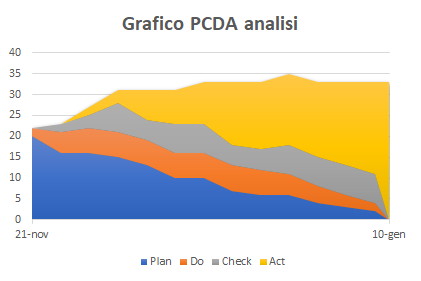
\includegraphics[scale=1]{Img/Grafico_PDCA}
	\caption{Grafico del metodo PDCA, fase di Analisi}\label{immagine:pdca analisi}
\end{figure}
Dal grafico possiamo estrapolare che:
\begin{itemize}
	\item alcuni dei processi pianificati hanno subito mutamenti, dovuti ad errori di pianificazione dati dalla poca esperienza del gruppo di lavoro;
	\item il gruppo ha reso l'avanzamento dei processi omogeneo, nonostante alcuni rallentamenti dovuti alla sovrapposizione di impegni personali e universitari dei componenti del gruppo con la realizzazione del progetto. Nel complesso si vede come l'omogeneità è stata abbastanza rispettata.
\end{itemize}
\subsubsection{Qualità di prodotto}
\paragraph{Indice di Gulpease} \Spazio
Vengono qui riportati i valori dell'indice Gulpease per ogni documento durante la fase di Analisi. 
\renewcommand{\arraystretch}{1.5}
\begin{table}[H]
\begin{center}
\begin{tabular}{|c|c|c|}
\hline
\rowcolor{title_row}
\textbf{\color{title_text}{Documento}} & \textbf{\color{title_text}{Valore indice}} & \textbf{\color{title_text}{Esito}} \\
\hline
	\emph{Piano di Progetto v1.0.0} & {55.49} & {Superato}\\
\hline
	\emph{Norme di Progetto v1.0.0} & {54.54} & {Superato}\\
\hline
	\emph{Analisi dei Requisiti v1.0.0} & {58.80} & {Superato}\\
\hline
	\emph{Piano di Qualifica v1.0.0} & {53.98} & {Superato}\\
\hline
	\emph{Studio di Fattibilità v1.0.0} & {50.77} & {Superato}\\
\hline
	\emph{Glossario v1.0.0} & {51.66} & {Superato}\\
\hline
\end{tabular}
\caption[Esiti verifica documenti, Analisi]{Indice di Gulpease per documento, fase di Analisi}
\label{tabella:verifica documenti}
\end{center}
\end{table}
\renewcommand{\arraystretch}{1}

Dalla tabella si può notare come tutti gli indici Gulpease dei documenti rientrino nei vincoli dati. Per questo motivo i documenti redatti hanno raggiunto la leggibilità desiderata.

\subsubsection{Dettaglio dell'esito della revisione}
\begin{itemize}
	\item\emph{Norme di Progetto}: sono state effettuate le integrazioni richieste ed è stata aggiornata la struttura del documento in modo da rispettare gli stessi standard per ogni sezione.\\
	La sottosezione relativa alla verifica è stata aggiornata in modo da contenere le nuove metriche inserite e le metriche erroneamente inserite nel \emph{Piano di Qualità v1.0.0}.	\item\emph{Analisi dei Requisiti}: sono state attuate le opportune modifiche suggerite. Alcuni casi d'uso sono stati leggermente rivisti ed è stato introdotto un caso d'uso più generico per ogni agglomerato di azioni con attitudini simili, modificando il caso d'uso principale. 	
	\item\emph{Piano di Progetto}: sono state fatte alcune verifiche nell'uso di alcuni termini e standard come consigliato dal committente. Sono stati aggiunte le opportune motivazioni e spiegazioni nelle scelte effettuate. La presentazione dei contenuti è stata rivista in modo da renderla più efficace.
	\item\emph{Piano di Qualifica}: il documento è stato profondamente rivisto per struttura e contenuti secondo quanto specificato dal committente.
	Le specifiche degli standard utilizzati e le descrizioni delle metriche sono stati spostati in appendice alle \emph{Norme di Progetto}. É stata aggiunta una sezione riguardante la pianificazione dei test, e le specifiche dei test sono state previste come futura aggiunta in appendice al documento. Infine, la strategia generale per la verifica ha assunto un ruolo centrale nella specifica degli obiettivi di qualità di processo e prodotto. 
\end{itemize}

\subsection{Revisione di Progettazione}
In questa sezione vengono riportati gli esiti delle metriche relative ai processi e delle metriche relative ai documenti.

\subsubsection{Qualità di processo}
\paragraph{Esiti metriche di processo}

\subparagraph{Consolidamento dei requisiti}\MiniSpazio
\renewcommand{\arraystretch}{1.5}
\begin{table}[H]
	\begin{center}
		\begin{tabular}{|c|c|c|}
			\hline
			\rowcolor{title_row}
			\textbf{\color{title_text}{Metrica}} & \textbf{\color{title_text}{Valore ottenuto}} & \textbf{\color{title_text}{Esito}} \\
			\hline
			{Schedule Variance} & {0} & {Superato}\\	
			\hline
			{Budget Variance} & {8\%} & {Superato}\\	
			\hline
		\end{tabular}
		\caption[Esiti metriche di processo, consolidamento dei requisiti]{Esiti derivanti dall'applicazione delle metriche di processo}	
		\label{tabella: esiti derivanti dall'applicazione delle metriche di processo cr}
	\end{center}
\end{table}


\subparagraph{Progettazione architetturale}\MiniSpazio
\renewcommand{\arraystretch}{1.5}
\begin{table}[H]
	\begin{center}
		\begin{tabular}{|c|c|c|}
			\hline
			\rowcolor{title_row}
			\textbf{\color{title_text}{Metrica}} & \textbf{\color{title_text}{Valore ottenuto}} & \textbf{\color{title_text}{Esito}} \\
			\hline
			{Schedule Variance} & {-3} & {Superato}\\	
			\hline	
			{Budget Variance} & {6\%} & {Superato}\\	
			\hline
			{Numero rischi non previsti} & {4} & {Superato}\\	
			\hline
			{Indisponibilità servizi esterni} & {0} & {Superato}\\	
			\hline
			{Media commit a settimana} & {26} & {Superato}\\	
			\hline
			{Media build Travis a settimana} & {22} & {Superato}\\	
			\hline
			{Percentuale build Travis superate} & {72.72\%} & {Superato}\\	
			\hline
		\end{tabular}
		\caption[Esiti metriche di processo, Progettazione Architetturale]{Esiti derivanti dall'applicazione delle metriche di processo}	
		\label{tabella: esiti derivanti dall'applicazione delle metriche di processo pa}
	\end{center}
\end{table}

\begin{figure} [H]
	\centering
	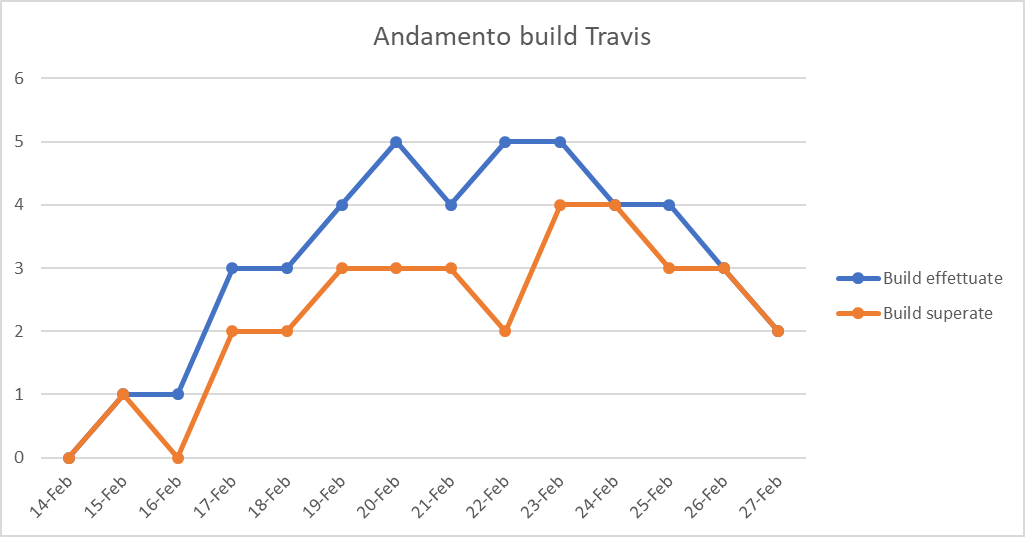
\includegraphics[scale=0.8]{Img/travis}
	\caption{Andamento delle build per il Proof of Concept}\label{}
\end{figure}

\paragraph{Maturità dei processi} \Spazio
Come riportato nella sezione 2.1.6, il gruppo adotta l'approccio a maturità di processo. Il livello di maturità assume valori da 1 a 5.

\subparagraph{Consolidamento dei requisiti}\MiniSpazio
\renewcommand{\arraystretch}{1.5}
\begin{table}[H]
	\begin{center}
		\begin{tabular}{|c|c|p{6.8cm}|}
			\hline
			\rowcolor{title_row}
			\textbf{\color{title_text}{Processo}} & \textbf{\color{title_text}{Livello di maturità}} & \textbf{\color{title_text}{Considerazioni}} \\
			\hline
			{Pianificazione e controllo} & {3} & {Gestito con l'ausilio di nTask, ha permesso di rispettare le scadenze previste.}\\	
			\hline
			{Gestione dei rischi} & {1} & {Non si sono verificate situazioni di rischio.}\\	
			\hline
			{Gestione dei test} & {0} & {Verrà istanziato una volta presente la necessità di definire e condurre dei test.}\\	
			\hline
			{Versionamento e build} & {0} & {Verrà istanziato una volta presente la necessità di versionare il prodotto software.}\\	
			\hline
		\end{tabular}
		\caption[Maturità dei processi, Consolidamento]{Maturità dei processi e considerazioni}	
		\label{tabella: considerazioni sulla maturità dei processi raggiunta}
	\end{center}
\end{table}
\pagebreak
\subparagraph{Progettazione architetturale}\MiniSpazio
\renewcommand{\arraystretch}{1.5}
\begin{table}[H]
	\begin{center}
		\begin{tabular}{|c|c|p{6.8cm}|}
			\hline
			\rowcolor{title_row}
			\textbf{\color{title_text}{Processo}} & \textbf{\color{title_text}{Livello di maturità}} & \textbf{\color{title_text}{Considerazioni}} \\
			\hline
			{Pianificazione e controllo} & {3} & {Ha permesso di rispettare le scadenze previste.}\\	
			\hline
			{Gestione dei rischi} & {1} & {Si è dimostrato poco stabile al verificarsi di 3 situazioni di rischio (malattia di membri del gruppo), comportando una ridefinizione degli obiettivi per il periodo.}\\	
			\hline
			{Gestione dei test} & {1} & {Sono stati pianificati i primi test di sistema, le cui specifiche tuttavia rimangono da definire.}\\	
			\hline
			{Versionamento e build} & {1} & {Parzialmente automatizzato con l'utilizzo dello strumento \gl{Travis}.}\\	
			\hline
		\end{tabular}
		\caption[Maturità dei processi, Progettazione Architetturale]{Maturità dei processi e considerazioni}	
		\label{tabella: considerazioni sulla maturità dei processi raggiunta pa}
	\end{center}
\end{table}
\renewcommand{\arraystretch}{1}

\paragraph{Dettaglio delle verifiche tramite analisi}
\subparagraph{Consolidamento dei requisiti}\MiniSpazio
Il grafico rappresentante l'applicazione del metodo PDCA nella fase di Consolidamento dei requisiti è:
\begin{figure} [H]
	\centering
	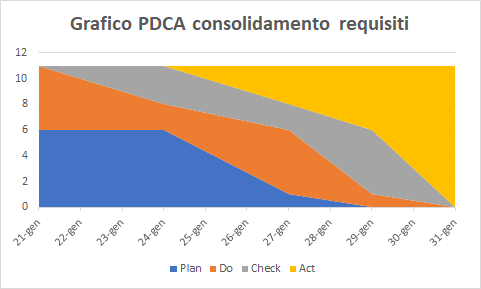
\includegraphics[scale=1]{Img/Grafico_PDCA_consolidamento_requisiti}
	\caption{Grafico del metodo PDCA, fase di Consolidamento dei requisiti}\label{}
\end{figure}
Dal grafico possiamo estrapolare che:
\begin{itemize}
	\item trattandosi di un periodo relativamente breve (10 giorni), piccole variazioni nel numero di attività risultano in grossi cambiamenti grafici;
	\item le attività in Plan sono state esaurite prima del termine del periodo, mentre quelle in Check e Act hanno avuto una permanenza maggiore; ciò é dovuto ad un numero di modifiche ai documenti relativamente basso ma di grande importanza e profondità (soprattutto per quanto riguarda il consolidamento del \emph{Piano di Qualifica}), che quindi hanno richiesto periodi di Check e Act prolungati.
\end{itemize}
\subparagraph{Progettazione architetturale}\MiniSpazio
Il grafico rappresentante l'applicazione del metodo PDCA nella fase di Progettazione architetturale è:
\begin{figure} [H]
	\centering
	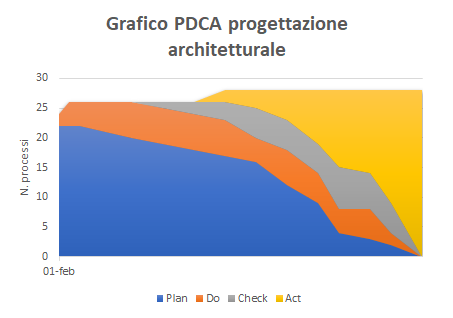
\includegraphics[scale=1]{Img/Grafico_PDCA_progettazione_architetturale}
	\caption{Grafico del metodo PDCA, fase di Progettazione architetturale}\label{}
\end{figure}
Dal grafico possiamo estrapolare che:
\begin{itemize}
	\item si nota uno stallo nell'esecuzione delle attività nella prima metà del periodo, dovuto principalmente, come previsto, alla sovrapposizione degli impegni universitari dei vari membri del gruppo. A questo si sono aggiunte le situazioni di rischio verificatesi, comportando ulteriori ritardi;
	\item verso al fine del periodo si nota un rapido decremento delle attività in Do e Check, dovuto ad uno sforzo maggiorato per compensare i ritardi dovuti alle situazioni di rischio verificatesi.
\end{itemize}
\subsubsection{Qualità di prodotto}
\paragraph{Indice di Gulpease} \Spazio
Vengono qui riportati i valori dell'indice Gulpease per ogni documento al termine della fase di Progettazione Architetturale.
\renewcommand{\arraystretch}{1.5}
\begin{table}[H]
	\begin{center}
		\begin{tabular}{|c|c|c|}
			\hline
			\rowcolor{title_row}
			\textbf{\color{title_text}{Documento}} & \textbf{\color{title_text}{Valore indice}} & \textbf{\color{title_text}{Esito}} \\
			\hline
			\emph{Piano di Progetto v2.0.0} & {53.78} & {Superato}\\
			\hline
			\emph{Norme di Progetto v2.0.0} & {53.87} & {Superato}\\
			\hline
			\emph{Analisi dei Requisiti v2.0.0} & {59.02} & {Superato}\\
			\hline
			\emph{Piano di Qualifica v2.0.0} & {49.68} & {Superato}\\
			\hline
			\emph{Studio di Fattibilità v2.0.0} & {49.64} & {Superato}\\
			\hline
			\emph{Glossario v2.0.0} & {52.11} & {Superato}\\
			\hline
		\end{tabular}
		\caption[Esiti verifica documenti, Consolidamento e Progettazione Architetturale]{Indice di Gulpease per documento, fase di Progettazione Architetturale}
		\label{tabella:verifica documenti rp}
	\end{center}
\end{table}
\renewcommand{\arraystretch}{1}
Dalla tabella si può notare come tutti gli indici Gulpease dei documenti rientrino nei vincoli dati. Per questo motivo i documenti redatti hanno raggiunto la leggibilità desiderata.

\begin{figure} [H]
	\centering
	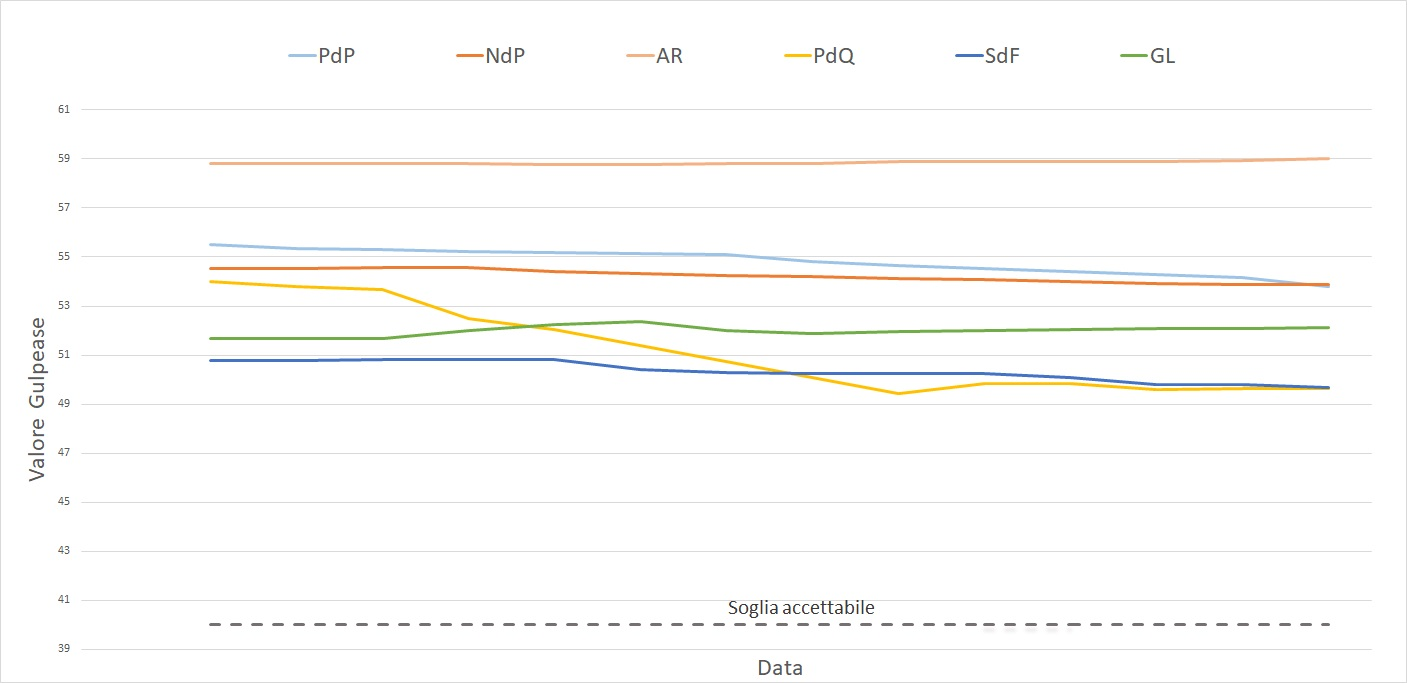
\includegraphics[scale=0.55]{Img/and_gulp_rp}
	\caption{Andamento dell'indice di Gulpease durante le fasi di Consolidamento dei requisiti e Progettazione architetturale}\label{immagine:gulpease rp}
\end{figure}

\pagebreak

\paragraph{Gunning fog index} \Spazio
\renewcommand{\arraystretch}{1.5}
\begin{table}[H]
	\begin{center}
		\begin{tabular}{|c|c|c|}
			\hline
			\rowcolor{title_row}
			\textbf{\color{title_text}{Documento}} & \textbf{\color{title_text}{Valore indice}} & \textbf{\color{title_text}{Esito}} \\
			\hline
			\emph{Piano di Progetto v2.0.0} & {13.21} & {Superato}\\
			\hline
			\emph{Norme di Progetto v2.0.0} & {12.74} & {Superato}\\
			\hline
			\emph{Analisi dei Requisiti v2.0.0} & {11.96} & {Superato}\\
			\hline
			\emph{Piano di Qualifica v2.0.0} & {12.87} & {Superato}\\
			\hline
			\emph{Studio di Fattibilità v2.0.0} & {11.18} & {Superato}\\
			\hline
			\emph{Glossario v2.0.0} & {14.39} & {Superato}\\
			\hline
		\end{tabular}
		\caption[Esiti verifica documenti, Consolidamento e Progettazione Architetturale]{Gunning fog index per documento, fase di Progettazione Architetturale}
		\label{tabella:verifica documenti gf}
	\end{center}
\end{table}
Dalla tabella si può notare come tutti gli indici Gunning fox dei documenti rientrino nei vincoli dati. Per questo motivo i documenti redatti hanno raggiunto la leggibilità desiderata.

\paragraph{Numero errori ortografici} \Spazio
Grazie le procedura di verifica e correzione attuate e all'ausilio dello strumento di controllo ortografico integrato in \gl{TexStudio}, il numero di errori ortografici per ogni documento ha raggiunto il valore ottimale di 0.

\section{Specifiche dei test}
Questa appendice contiene le specifiche relative ai vari test pianificati. Verrà redatta una volta presente la necessità di eseguire tali test.
